
% this file is called up by thesis.tex
% content in this file will be fed into the main document

%: ----------------------- introduction file header -----------------------
%\begin{savequote}[50mm]
%Historical methodology, as I see it, is a product of common sense applied to circumstances. 
%\qauthor{Samuel E. Morison}
%\end{savequote}


\chapter{Método para la evaluación de competencias genéricas}
\label{cha:Overall methodology}

% the code below specifies where the figures are stored
\ifpdf
    \graphicspath{{4_overall_methodology/figures/PNG/}{4_overall_methodology/figures/PDF/}{4_overall_methodology/figures/}}
\else
    \graphicspath{{4_overall_methodology/figures/EPS/}{4_overall_methodology/figures/}}
\fi

%------------------------------------------------------------------------- 

En este capítulo se propone un método para la evaluación de competencias genéricas de los estudiantes basado en el diseño de evaluaciones a partir de la actividad de estos en los entornos de aprendizaje. Se describen el método, sus características, la adecuación del método para satisfacer los requisitos deseados y se introduce el tipo de herramienta que se empleará para su implementación.

\section{Introducción}

Prácticamente hoy en día los LMS constituyen una pieza fundamental en cualquier contexto en el que se impartan cursos. Mientras que en los cursos virtuales los LMS son el único entorno de trabajo posible, en los cursos presenciales o mixtos, tantos los LMS como otros entornos virtuales de aprendizaje actúan como soporte virtual de las clases, proporcionando multitud de actividades de aprendizaje. 

En esta tesis se propone un método de evaluación de competencias genéricas basado en el diseño de evaluaciones (DBA, del inglés, \emph{design-based assessment}) y que tiene su origen en la investigación basada en el diseño (DBR). DBA es un método de evaluación de competencias genéricas que se basa en el diseño de indicadores a partir de la actividad generada por los estudiantes en los entornos virtuales de aprendizaje. Los docentes podrán diseñar evaluaciones utilizando estos indicadores y podrán utilizar estas evaluaciones como evidencias del desempeño de competencias genéricas. Si llegado el caso, el docente considera que las evidencias no terminan de reflejar bien el desempeño de las competencias, el método DBA le permitirá refinar los diseños hasta llegar a unas evidencias que sí le sean válidas, o a descartarlas si no llegaran a serlas. Además, los diseños podrán ser utilizados y modificados por otros docentes que busquen adaptarlos a su contexto local o a las competencias genéricas que deseen medir. 

En el LMS por ejemplo, los estudiantes acceden a su contenido a diario. Por un lado, habrá estudiantes que accedan al LMS cada día a consultar novedades, participar en foros, subir tareas o descargar apuntes, mientras que por otro lado, habrá estudiantes que entren sólo de manera puntual, a realizar un examen o a subir una tarea. Todas las acciones quedan almacenadas en el registro de actividad de los LMS, y estos registros podrían ser analizados para comprender el proceso de aprendizaje que se está desarrollando mediante técnicas de \emph{learning analytics}. El método DBA se basa en la utilización e integración de técnicas y herramientas de \emph{learning analytics} para la obtención de información del registro de actividad procedente de estos y otros entornos virtuales de aprendizaje con los que diseñar indicadores.

% Revisar párrafo anterior sobre el contexto de learning analytics

\section{Método: design-based assessment (DBA)} \label{cha:met-sec:dba}

En esta sección se explica el método de evaluación DBA. La sección comienza con un apartado dedicado a la contextualización del método y continúa con la descripción en detalle del mismo.

\subsection{Contexto}

Los estudiantes comienzan a dejar constancia de su actividad en los entornos virtuales de aprendizaje desde el momento en que acceden al entorno. El registro del sistema almacena gran cantidad de información, tanto la participación activa del estudiante, cuando éste interactúa con el entornos virtuales de aprendizaje, como la participación pasiva, cuando el estudiante simplemente accede y navega entre sus contenidos. 

Los docentes pueden plantear actividades en los entornos virtuales de aprendizaje con la intención no sólo de evaluar ciertas habilidades de los estudiantes, sino también de provocar comportamientos en los estudiantes y ver cómo afrontan ciertas situaciones. Pueden encontrarse patrones de comportamiento en la manera en que los estudiantes abordan ciertas tareas y estos comportamientos podrían ser interpretados como un indicador del desempeño de alguna competencia genérica.

Los guías docentes de las asignaturas incluyen las competencias genéricas de las que los estudiantes deben ser evaluados. Para evaluar una competencia genérica dada, el docente puede diseñar una evaluación a partir de la información relativa a los registros de los entornos de aprendizaje. Aquí comienza un \emph{ciclo de contraste de hipótesis}. 

\subsection{Descripción del método}

El método DBA es iterativo, ya que permite al docente rediseñar y contrastar hipótesis y resultados hasta confirmar la hipótesis, o por el contrario, descartarla y enunciar una nueva. Podemos decir que el método se integra en un \emph{ciclo de contraste de hipótesis}. Este ciclo consta de una serie de pasos que se muestran en la figura~\ref{fig:CCHDiagram} y se explican a continuación:

\begin{figure}
  \begin{center}
    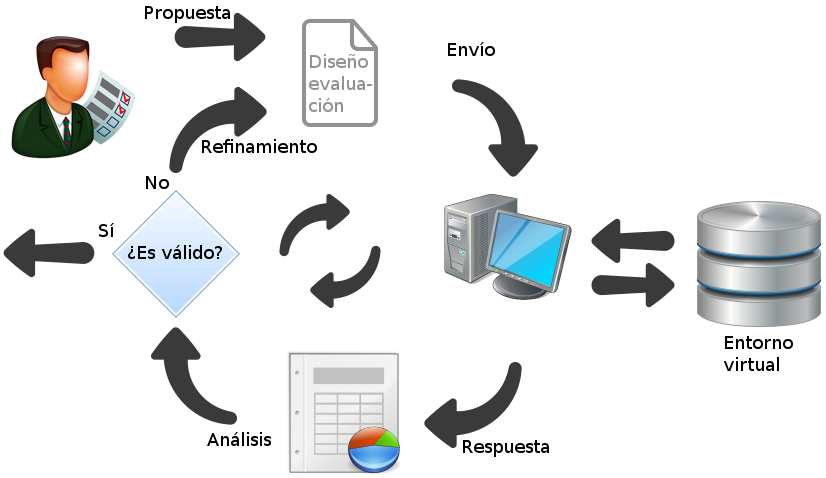
\includegraphics[scale=0.45]{CCHDiagram.png}
  \end{center}
  \caption{Diagrama del ciclo de contraste de hipótesis}
  \label{fig:CCHDiagram}
\end{figure}

\begin{enumerate}
\item \emph{Hipótesis inicial}: el docente formula una hipótesis de partida para la utilización de algún tipo de información de la actividad de los estudiantes en el entorno virtual de aprendizaje para la evaluación de alguna competencia genérica (a). Por ejemplo, se considerará que un estudiante tiene un desempeño correcto de la competencia genérica de planificación y gestión del tiempo si entrega las tareas programadas por el docente en el entorno virtual con anterioridad a la fecha fijada para las mismas.
\item \emph{Diseño y formulación de evaluación}: el docente diseña un indicador para evaluar la competencia a partir de la información del registro y la implementará en la herramienta utilizada para extraer la información (b). Por ejemplo, podríamos considerar partiendo de la hipótesis anterior que un estudiante tendrá un desempeño alto en la competencia de planificación y gestión del tiempo si de las 10 tareas programadas durante el semestre al menos 9 fueron entregadas antes de la fecha fijada para las mismas, un desempeño medio si entregó entre 7 y 8 tareas antes de la fecha fijada y un desempeño bajo si entregó 6 o menos tareas antes de la fecha fijada.
\item \emph{Petición de datos}: se envía la petición de datos al sistema encargado de recuperar la información (c). Las herramientas y su funcionamiento serán explicadas más adelante en la sección~\ref{cha:met-sec:tools}.
\item \emph{Validación de resultados}: la herramienta pondrá a disposición del docente los indicadores requeridos (d). El docente los analizará (e) y evaluará si son válidos para el propósito que fueron diseñados, si necesitan ser refinados o si hay que descartarlos (f). En este caso, podrá volver al segundo punto y rediseñar una nueva evaluación (g).
\end{enumerate}

A continuación se presentara un ejemplo para ilustrar el ciclo de contraste de hipótesis. 

\subsubsection*{Ejemplo de ciclo de contraste de hipótesis}

En este ejemplo, el docente pretende obtener indicadores del uso del foro del LMS para evaluar la competencia genérica de las habilidades interpersonales. Durante el curso, el docente planteó una actividad de debate mediante el foro de la asignatura que tuvo lugar durante una semana de las que conforman el curso. El docente aplicará dos iteraciones del ciclo de contraste de hipótesis del método DBA.

\paragraph*{Iteración I}

\subparagraph*{I.1 Hipótesis inicial.}

El docente considera que podría diseñar un indicador válido a partir del número de mensajes que ha escrito cada estudiante en la semana en la que transcurre la actividad y plantea la siguiente hipótesis: \emph{se considerará que un estudiante ha desempeñado satisfactoriamente la competencia genérica de las habilidades interpersonales si ha escrito al menos dos mensajes en el foro en la semana}.

\subparagraph*{I.2 Diseño y formulación de la evaluación.}

Para diseñar la evaluación, el docente deberá contar con un lenguaje cercano al dominio que le permita formular la consulta que le proporcione los indicadores que requiere la hipótesis inicial. En este ejemplo mostramos la consulta I.1, escrita en el lenguaje SASQL~\footnote{https://www.assembla.com/spaces/evalcourse/wiki/SASQL} (que se presenta en la sección~\ref{subcha:evc}) y que proporcionará datos sobre la participación de los estudiantes en el foro entre dos fechas.

\begin{minted}[label=Consulta I.1,
		linenos,
		frame=lines,
               	framesep=2mm]{sql}
Evidence participacion_foro: 
	get students
	show participation
	in forum between 2015-10-21 and 2015-10-27.
\end{minted}


\subparagraph*{I.3 Petición de datos.}

En este paso, se enviará la consulta a un software que lo interprete, procese y sea capaz de proporcionar los datos solicitados. %La consulta anterior se introduciría en el software EvalCourse, herramienta creada para este trabajo que acepta consultas escritas en SASQL y se conecta al entorno virtual de aprendizaje.

\subparagraph*{I.4 Validación de resultados.}

El software devuelve al docente los indicadores solicitados mediante el listado~\ref{tab:EvalCourseEj1}. El docente los analiza y concluye que, en base a la hipótesis inicial, todos los estudiantes menos el 3 (\emph{student3}) habrían desempeñado correctamente la competencia. Sin embargo, el docente considera pobre esta primera aproximación y decide redefinir la hipótesis inicial.

\begin{table}
	\centering
	\caption{Información sobre la participación en el foro de los estudiantes en un periodo concreto de tiempo}
	\label{tab:EvalCourseEj1}
	\begin{tabular}{|l|l|c|c|c|c|c|}
		\hline
		id & username & Debate-starter & Debate-participation & Total \\
		\hline
		\hline
		1 & student1 & 1 & 2 & 3  \\
		\hline
		2 & student2 & 0 & 4 & 4  \\
		\hline
		3 & student3 & 0 & 1 & 1  \\
		\hline
		4 & student4 & 1 & 2 & 3  \\
		\hline
		5 & student5 & 0 & 2 & 2  \\
		\hline
	\end{tabular}
\end{table}


\paragraph*{Iteración II}

\subparagraph*{II.1 Hipótesis inicial.}

El docente plantea la nueva hipótesis inicial de la siguiente manera: \emph{se considerará que un estudiante ha desempeñado satisfactoriamente la competencia genérica de las habilidades interpersonales si ha escrito al menos dos mensajes en el foro y ha interactuado con más de un compañero en la semana}.

\subparagraph*{II.2 Diseño y formulación de la evaluación.}

El docente diseña la nueva evaluación mediante la consulta SASQL I.2.

\begin{minted}[label=Consulta I.2,
		linenos,
		frame=lines,
               	framesep=2mm]{sql}
Evidence interacciones_foro: 
	get students
	show interaction
	in forum between 2013-10-21 and 2013-10-27.
\end{minted}

\subparagraph*{II.3 Petición de datos.}

Se ejecuta la consulta en el software.

\subparagraph*{II.4 Validación de resultados.}

El software devuelve, entre otros formatos, un grafo que muestra las interacciones (figura~\ref{fig:EvalCourseInteraccionForo}). A tenor de los resultados se observa que sólo dos de los estudiantes cumplen la segunda hipótesis (\emph{student2} y \emph{student4}), y bajo esta nueva hipótesis, ellos serían los dos únicos estudiantes que han mostrado un buen desempeño de la competencia genéricas de las habilidades interpersonales.

\begin{figure}
	\centering
	\includegraphics[width=6cm]{{EvalCourseInteraccionForo.png}}
	\caption{Interacción en el foro en un periodo de tiempo.}
	\label{fig:EvalCourseInteraccionForo}
\end{figure}

\section{Características, requisitos y herramienta} \label{cha:met-sec:req}

El método DBA para la evaluación de competencias genéricas es un método DBR. Aunque desde el punto de vista del estudiante y considerando la clasificación de métodos de evaluación mostrada en la sección~\ref{sec:methods} diríamos que es un método \emph{evaluación formativo}, ya que permite mejorar el aprendizaje mientras este tiene lugar proporcionando información de manera sistemática y continua. Sin embargo, lo consideramos un método DBR ya que no mejora únicamente la acción del alumno, sino que también es un método de investigación que mejora la acción del docente.

Mientras que con respecto a la clasificación de técnicas de evaluación mostrada en la sección~\ref{sec:techniques}, la técnica empleada en este método es la de obtención de \emph{indicadores del trabajo en actividades de aprendizaje}.

\subsection{Características}

En el capítulo de la introducción se indican, partiendo del análisis realizado por Terry Andersen y Julie Shattuck~\cite{anderson2012design}, las características que un estudio DBR de calidad debe tener. A continuación se identificará nuestro método DBA en cada una de esas características:

\begin{itemize}
\item \emph{Estar situado en un contexto educativo real}: el método DBA se ha creado en un contexto educativo real (la Universidad de Cádiz) para ser utilizado en este y en otros contextos educativos reales. Su validez será tratada en el capítulo de la evaluación.
\item \emph{Enfocado en el diseño y prueba de una intervención significativa}: La intervención que se lleva a cabo con el método DBA es un \emph{tipo de evaluación}, siendo este uno de los tipos de intervenciones recogidos en la tipología de intervenciones DBR definida por Andersen~\cite{anderson2012design}. 
\item \emph{Empleo de métodos mixtos}: una intervención DBR implica normalmente la aplicación de diferentes métodos, técnicas y herramientas. El método DBA puede combinarse con otros métodos de evaluación con el fin de contrastar evaluaciones y dar validez a los resultados obtenidos con uno u otro método. Por ejemplo, una aplicación de métodos mixtos podría darse en el ejemplo mostrado en el apartado anterior, donde los estudiantes eran evaluados de sus habilidades interpersonales mediante el método DBA. Esa actividad podría formar parte de un conjunto de actividades de trabajo en equipo configuradas por el docente para realizar una evaluación auténtica. El docente podría combinar los resultados de la aplicación de ambos métodos y así contrastar los resultados.
\item \emph{Múltiples iteraciones}: el método DBA permite el diseño de evaluaciones y su contraste de resultados (\emph{ciclo de contraste de hipótesis}). A partir de los resultados, el diseño se puede ir refinando iterativamente hasta que los resultados satisfagan las expectativas del docente o hasta que decida descartarlos por no ser válidos para su evaluación.
\item \emph{Asociación colaborativa entre investigadores y docentes}: el proceso de desarrollo de software es cada vez más colaborativo, tratando de integrar todo lo posible a los usuarios finales para avanzar hacia un proceso dirigido por la comunidad donde tanto los actores técnicos como los no técnicos trabajen juntos para que se cumplan las expectativas. Esto es especialmente apropiado en el campo de los DSL, herramientas informáticas diseñadas para facilitar el desarrollo de software en un contexto específico~\cite{izquierdo2012community}. Bajo este enfoque se desarrollará el método DBA, colaborando docentes e investigadores en su desarrollo, teniendo así los usuarios finales y expertos en el dominio (los docentes) una participación activa y directa en la definición de una herramienta que implemente el método, es decir, un DSL. 
\item \emph{Evolución de los principios de diseño}: el método DBA permite la creación de diseños para aplicar a diferentes competencias. Ciertos diseños podrían ser definidos como plantillas o patrones para la evaluación de competencias. Estos patrones podrán ser utilizados por otros docentes, y a partir de su reflexión, modificados para  adaptarlos a nuevos contextos. De esta forma, los principios y diseños creados por docentes e investigadores no mueren con una práctica, sino que son puntos de partidas para nuevas teorías y experimentos. Por ejemplo, un docente que trabajase con wikis en sus clases podría utilizar como indicador de desempeño de la competencia de trabajo en equipo el número de contribuciones realizado por cada estudiante a la página de su equipo. Un segundo docente que trabajase con wikis podría mejorar esta evaluación considerando como indicador el peso en bytes de las contribuciones aportadas por cada miembro del equipo. Y un tercer docente podría mejorar esta evaluación añadiendo una restricción temporal a la información aportada al wiki por cada miembro del equipo. Es decir, se parte de un patrón o diseño inicial que los docentes han ido evolucionando para mejorarlo y aplicarlo a su contexto.
\item \emph{Comparación con la investigación-acción}: el objetivo del método DBA, al contrario de lo que ocurre con la investigación-acción, no es sólo alcanzar una serie de objetivos a nivel local, sino que también permite evolucionar a nivel teórico y maximizar la generalización, mejorando así la comprensión de aplicaciones prácticas. Además, permite la participación de un equipo formado por investigadores y docentes mientras que, por lo general, la práctica de la investigación-acción es llevada a cabo únicamente por el docente que realiza el experimento. Ambos enfoques son muy parecidos y en ocasiones cuesta diferenciarlos. Se podría decir que la investigación-acción carece de ese carácter reflexivo que sí tiene el DBR~\cite{cole2005being}. Para ilustrarlo utilizaremos el ejemplo de la medición de la competencia de trabajo en equipo mediante el wiki mostrado en el punto anterior. En la investigación-acción, un docente se enfrentaría a esta evaluación por sí solo, sin considerar cómo han evaluado dicha competencia otros en el wiki, sino que adoptaría una solución útil para él en su caso pero que no evolucionaría. Justo al contrario de lo que ocurrió en el ejemplo anterior de wikis, donde cada docente, investigador o equipo de investigadores y/o docentes tenía en cuenta como había sido abordada antes la evaluación del trabajo en equipo en el wiki y cada nueva evaluación se pudo utilizar como base de futuras evaluaciones.
\item \emph{Repercusión en las prácticas}: el método DBA puede repercutir directamente en las prácticas. A partir de su aplicación en la docencia práctica y del análisis de resultados, los investigadores y docentes implicados pueden detectar actividades e interacciones que favorecen el desempeño de competencias y que no habían considerado anteriormente. Esto repercutirá directamente en la organización y programación de actividades en los siguientes cursos.
\end{itemize}

\subsection{Requisitos}

En el capítulo~\ref{cha:Problemas} se enumeraron los requisitos que el método deberá cumplir. A continuación se indica cómo el método, apoyado en la herramienta que lo implementa, abordan cada uno de estos requisitos.

\paragraph*{1. Indicadores objetivos}

Los indicadores que se obtienen con el método DBA reflejan valores de los registros de actividad del entorno virtual de aprendizaje. Por tanto, son objetivos en cuanto a que dos estudiantes que tienen los mismos valores en el registro tendrán en el mismo valor en el indicador, y ya será decisión del docente la interpretación de este indicador.

\paragraph*{2. Evaluación escalable}

El método DBA se alinea con las actividades de aprendizaje para que el docente pueda obtener los indicadores del registro para todos o parte de los estudiantes de un curso con una simple petición a la herramienta, sin importar el número de estudiantes.

\paragraph*{3. Propósito general}

El método DBA permite obtener indicadores de la actividad de los estudiantes en el entorno de aprendizaje virtual. Estos indicadores no están asociados a ninguna competencia específica, es información objetiva almacenada directamente en la base de datos del entorno y puesta, mediante la herramienta que implemente el método, a disposición del docente. Por tanto, se puede afirmar que el método DBA es de propósito general pues será el docente quién deba valorar para la evaluación de qué competencia lo podrá utilizar en cada caso.

\paragraph*{4. Accesibilidad}

La información del registro de actividad del entorno virtual está contenida en la base de datos del entorno. Pero ni los docentes suelen tener acceso a dicha base de datos, ni aún teniéndolo tienen que saber utilizar el lenguaje de acceso a bases de datos (SQL) para realizar las consultas a las tablas que contienen la información. Con el fin de poder obtener los indicadores de una forma que sea accesible y utilizable por docentes sin conocimientos de programación, la herramienta que lo implemente debe ser un lenguaje de consultas sencillo que les permita definir las evaluaciones. El lenguaje tiene una sintaxis con términos del dominio de la docencia, de manera que este tipo de docentes pueda utilizarlo. El docente realizará la consulta y, la herramienta ya conectada a la información, le proporciona los valores de los indicadores en diferentes formatos abiertos que el docente podrá visionar y exportar a otras herramientas. \nomenclature{SQL}{Structured Query Language}

\paragraph*{5. Diseño de evaluaciones}

El método DBA, mediante el lenguaje de consultas mencionado en el punto anterior, permitirá a los docentes ejercer una labor de diseñador de evaluaciones, utilizando y combinando la información obtenida del entorno de aprendizaje para calcular indicadores que aplicar a las competencias genéricas para las que ellos consideren que les son válidos.

\subsection{Herramienta} \label{cha:met-sec:tools}

La herramienta que implemente el método debe tener una serie de características que derivan de los requisitos mencionados anteriormente y que son los siguientes:

\begin{itemize}
%\item \emph{Conectada al entorno virtual de aprendizaje}: para poder extraer los registros de actividad de los entornos virtuales de aprendizaje, la herramienta debe conectarse a dichos entornos.
\item \emph{Personalización de evaluaciones}: la herramienta debe proporcionar un mecanismo para permitir al usuario crear sus diseños a partir de los indicadores disponibles en el entorno virtual de aprendizaje. Para permitir al usuario definir los diseños se decide que la herramienta sea un lenguaje de consultas.
\item \emph{Cercano al dominio}: el lenguaje debe servir al docente o investigador para definir indicadores a partir de la actividad de los estudiantes en los entornos de aprendizaje, por tanto, debe ser un lenguaje cuya sintaxis esté definida en términos del ámbito educativo.
\item \emph{Usabilidad}: el lenguaje debe ser usable por usuarios de perfil no informático, por lo que su utilización debe ser sencilla y entendible por este tipo de usuarios.
\end{itemize}

A tenor de estos requisitos se decidió que la herramienta informática a implementar sería un \emph{lenguaje específico de dominio} (DSL). Un DSL es un lenguaje de programación orientado a un dominio concreto. Estos se han vuelto muy populares en los últimos años, y una de las principales razones es que facilitan la comunicación con los expertos en el dominio, proporcionando un texto común (código escrito en el DSL) que actúa a la vez como ejecutable y como una descripción que los expertos en el dominio pueden leer para entender como sus ideas se representan en el sistema~\cite{fowler2010domain}. En el método DBA, el ejecutable sería el diseño y los expertos en el dominio los docentes.



% La evaluación de las 3 herramientas se corresponde al capítulo siguiente.


%Metodología mixta

%Cómo voy a evaluar roles, momentos, actividad, ... lo que sea.

%Explicar el DSL

%DSL: herramienta de investigación en evaluaciones. Esta herramienta ayuda al investigador a formalizar la evaluación.
 
%Enfocar la metodología a que no es una metodología para evaluar, sino para diseñar evaluaciones. Diseñador de evaluaciones.

%Explicar qué pasos tiene que seguir un diseñador de evaluaciones para hacer sus evaluaciones.

%Dentro de los resultados obtenemos dos cosas:
%1. Diseño
%2. Lo que el diseñador nos indicó que no pudo hacer

%Para que esto sea posible falta la herramienta informática

%\section{Evolución herramientas}

%AMW --> EvalCourse --> EvalSim

%\section{Metodología de desarrollo}

%DSL? Ing. Dirigida x modelo?



%------------------------------------------------------------------------------------------------------------------------------------------------

